\documentclass[border=10pt]{standalone}
\usepackage{tikz,amsmath}
\usetikzlibrary{arrows.meta,3d}

% ========== 颜色定义 ==========
\colorlet{myred}{red!80!black}
\colorlet{myblue}{blue!80!black}
\colorlet{mygreen}{green!60!black}
\colorlet{myorange}{orange!70!red!60!black}

\begin{document}
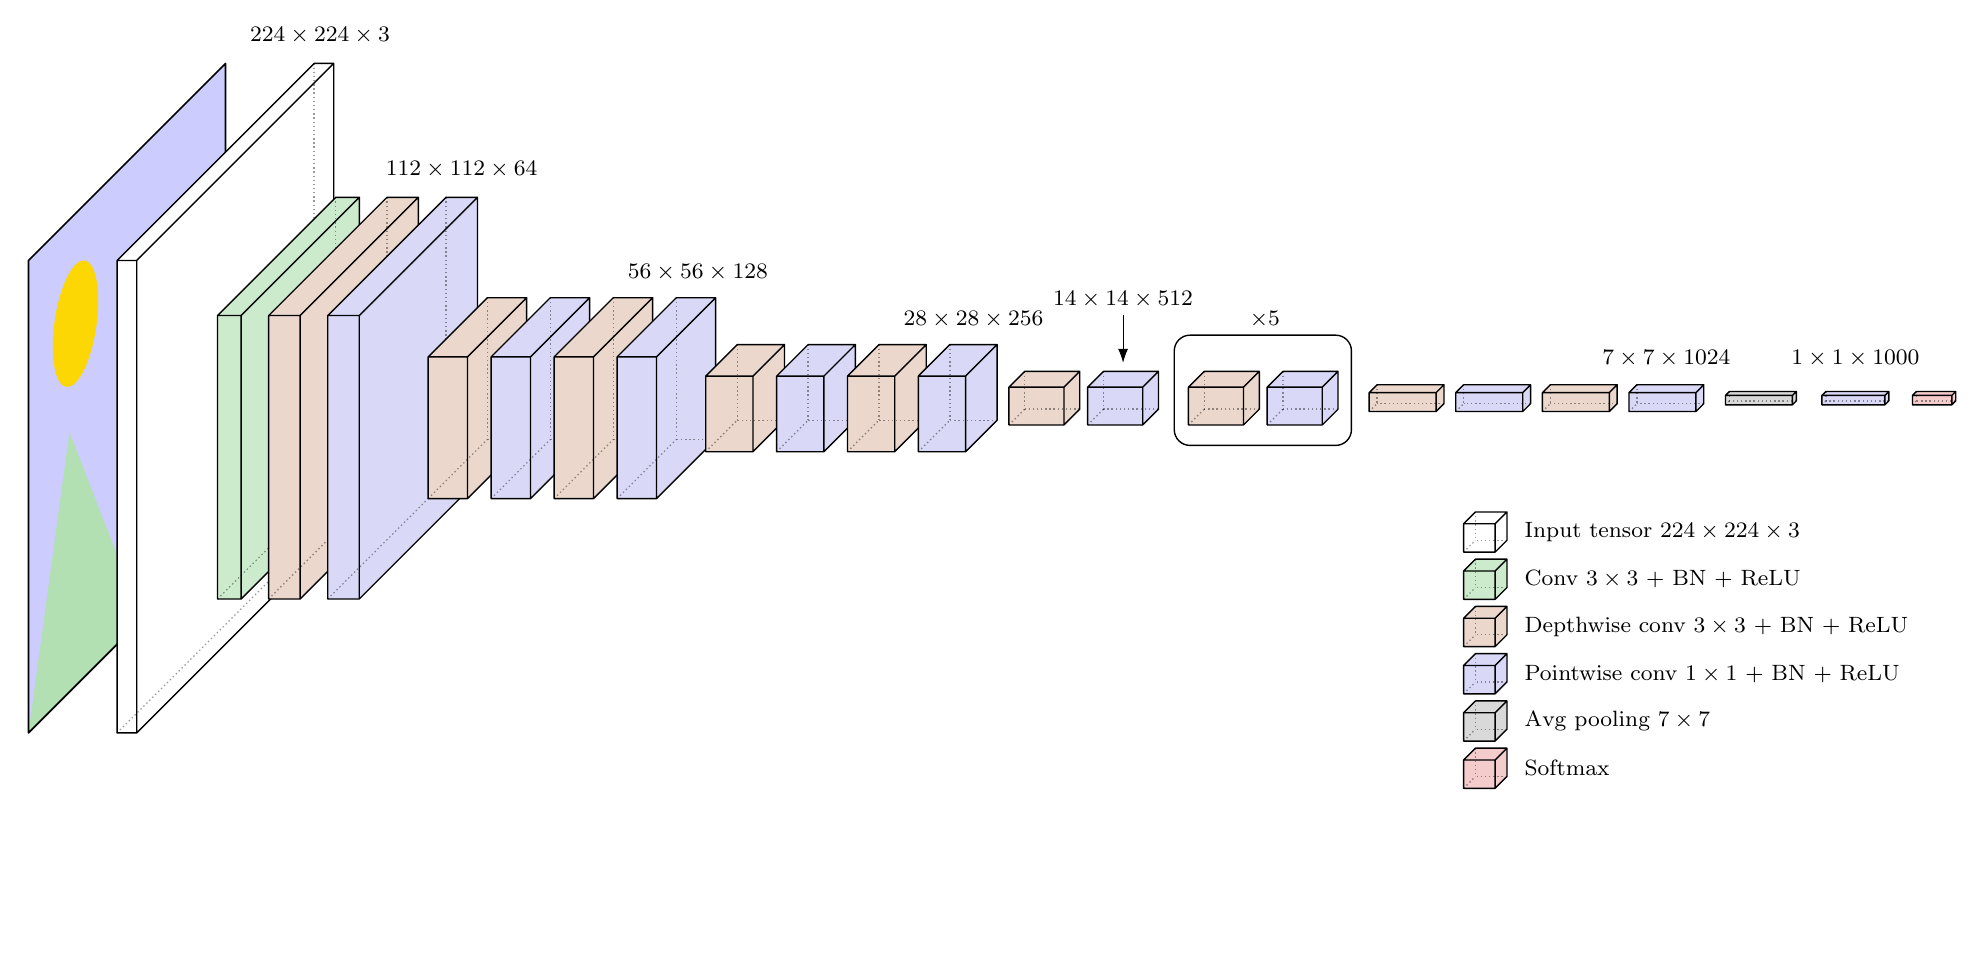
\begin{tikzpicture}[
    font=\footnotesize, scale=1, line join=round,
    every node/.style={outer sep=0pt, inner sep=0pt, align=center},
    >={Latex[length=1.75mm, width=1.25mm]}
  ]

  % ========== 立方体绘制宏 ==========
  \def\cube#1#2#3#4#5#6#7{%
    \begin{scope}[shift={(#1,#2)},scale=1]
      \pgfmathsetmacro{\cubex}{#4}
      \pgfmathsetmacro{\cubey}{#5}
      \pgfmathsetmacro{\cubez}{#6}
      \draw [draw=black, line width=.5pt,
             every edge/.append style={draw=black, opacity=.4, densely dotted},
             fill=#7, fill opacity=1]
        (\cubex/2,\cubey/2,\cubez/2) coordinate (o)
          -- ++(-\cubex,0,0) coordinate (a)
          -- ++(0,-\cubey,0) coordinate (b)
            edge coordinate [pos=1] (g) ++(0,0,-\cubez)
          -- ++(\cubex,0,0) coordinate (c) -- cycle
        (o) -- ++(0,0,-\cubez) coordinate (d)
          -- ++(0,-\cubey,0) coordinate (e) edge (g) -- (c) -- cycle
        (o) -- (a) -- ++(0,0,-\cubez) coordinate (f) edge (g) -- (d) -- cycle;
      \node[rotate=90, xshift=-2cm, yshift=.165cm] {#3};
    \end{scope}
  }

  % ========== 输入图像（zy 平面）==========
  \begin{scope}[canvas is zy plane at x=0.25, transform shape]
    \fill[blue!20] (-3.25,-3) rectangle (3.25,3);
    \fill[yellow!75!orange] (1.7,1.6) circle (.75);
    \fill[green!50!black!45] (-3.25,-3) -- (-1.1,.9) -- (.9,-3) -- cycle;
    \fill[green!60!black!30] (-.5,-3) -- (1.9,.3) -- (3.25,-3) -- cycle;
    \draw[black, line width=.6pt] (-3.25,-3) rectangle (3.25,3);
  \end{scope}

  % ========== 立方体序列 ==========
  % Input: 224x224x3
  \cube{1.5}{0}{}{.25}{6}{6.5}{white}

  % Conv3x3 (s2): 112x112x32
  \cube{2.3}{0}{}{.3}{6*.6}{6.5*.6}{mygreen!20}

  % Block 1 (s1): 112x112x64
  \cube{3.0}{0}{}{.4}{6*.6}{6.5*.6}{myorange!20}
  \cube{3.75}{0}{}{.4}{6*.6}{6.5*.6}{myblue!15}

  % Block 2 (s2): 56x56x128
  \cube{4.7}{0}{}{.5}{6*.3}{6.5*.3}{myorange!20}
  \cube{5.5}{0}{}{.5}{6*.3}{6.5*.3}{myblue!15}
  % Block 3 (s1): 56x56x128 (新增)
  \cube{6.3}{0}{}{.5}{6*.3}{6.5*.3}{myorange!20}
  \cube{7.1}{0}{}{.5}{6*.3}{6.5*.3}{myblue!15}

  % Block 4 (s2): 28x28x256
  \cube{8.1}{0}{}{.6}{6*.16}{6.5*.16}{myorange!20}
  \cube{9.0}{0}{}{.6}{6*.16}{6.5*.16}{myblue!15}
  % Block 5 (s1): 28x28x256 (新增)
  \cube{9.9}{0}{}{.6}{6*.16}{6.5*.16}{myorange!20}
  \cube{10.8}{0}{}{.6}{6*.16}{6.5*.16}{myblue!15}

  % Block 6 (s2): 14x14x512
  \cube{11.9}{0}{}{.7}{6*.08}{6.5*.08}{myorange!20}
  \cube{12.9}{0}{}{.7}{6*.08}{6.5*.08}{myblue!15}
  % Blocks 7-11 (s1 x 5): 14x14x512
  \cube{14.18}{0}{}{.7}{6*.08}{6.5*.08}{myorange!20}
  \cube{15.18}{0}{}{.7}{6*.08}{6.5*.08}{myblue!15}
  \draw[black, line width=.5pt, rounded corners=2mm] (13.55,-.6) rectangle (15.8,0.8);
  \node at (14.7,1.0) {$\times 5$};

  % Block 12 (s2): 7x7x1024
  \cube{16.5}{0}{}{.85}{6*.04}{6.5*.04}{myorange!20}
  \cube{17.6}{0}{}{.85}{6*.04}{6.5*.04}{myblue!15}
  % Block 13 (s1): 7x7x1024 (新增)
  \cube{18.7}{0}{}{.85}{6*.04}{6.5*.04}{myorange!20}
  \cube{19.8}{0}{}{.85}{6*.04}{6.5*.04}{myblue!15}

  % Head: AvgPool + FC/Conv1x1 + Softmax
  \cube{21.0}{0}{}{.85}{6*.02}{6.5*.02}{gray!30}
  \cube{22.2}{0}{}{.8}{6*.02}{6.5*.02}{myblue!15}
  \cube{23.2}{0}{}{.5}{6*.02}{6.5*.02}{myred!20}

  % ========== 图例 ==========
  \cube{17.5}{-1.7}{}{.4}{6*.06}{6.5*.06}{white}
  \cube{17.5}{-2.3}{}{.4}{6*.06}{6.5*.06}{mygreen!20}
  \cube{17.5}{-2.9}{}{.4}{6*.06}{6.5*.06}{myorange!20}
  \cube{17.5}{-3.5}{}{.4}{6*.06}{6.5*.06}{myblue!15}
  \cube{17.5}{-4.1}{}{.4}{6*.06}{6.5*.06}{gray!30}
  \cube{17.5}{-4.7}{}{.4}{6*.06}{6.5*.06}{myred!20}
  \node[anchor=west] at (18.0,-1.7) {Input tensor $224\times224\times3$};
  \node[anchor=west] at (18.0,-2.3) {Conv $3\times3$ + BN + ReLU};
  \node[anchor=west] at (18.0,-2.9) {Depthwise conv $3\times3$ + BN + ReLU};
  \node[anchor=west] at (18.0,-3.5) {Pointwise conv $1\times1$ + BN + ReLU};
  \node[anchor=west] at (18.0,-4.1) {Avg pooling $7\times7$};
  \node[anchor=west] at (18.0,-4.7) {Softmax};

  % ========== 尺寸标注 ==========
  \node at (2.7,4.6) {$224 \times 224 \times 3$};
  \node at (4.5,2.9) {$112 \times 112 \times 64$};
  \node at (7.5,1.6) {$56 \times 56 \times 128$};
  \node at (11.0,1.0) {$28 \times 28 \times 256$};
  \node at (12.9,1.25) {$14 \times 14 \times 512$};
  \draw[line width=.3pt, ->] (12.9,1.05) -- (12.9,0.45);
  \node at (19.8,0.5) {$7 \times 7 \times 1024$};
  \node at (22.2,0.5) {$1 \times 1 \times 1000$};

\end{tikzpicture}
\end{document}